\ifgerman{\chapter{Grundlagen}}{\chapter{Background}}
\label{ch:background}

This chapter covers the fundamentals of document classification, how machine learning can be applied for document classification. Furthermore, this chapter will provide an overview of various machine learning, deep learning, and evaluation concepts.  This chapter will also describe the concepts of different classification algorithms employed. 

\section{Document Categorization}
Due to the internet, we have access to an enormous amount of resources online. Governments, universities and other organizations regularly publish new documents which are hard to oversee. Organization and categorization of these documents are therefore important now more than ever. Due to organizations operating in different geographies, documents publish by them are available in multiple languages and are from different domains which make it more difficult to categorize and retrieve them. For example, the European Union publishes the documents in all the 24 official languages, big multinational companies like Volkswagen cars are present in 153 countries\footnote{https://www.volkswagenag.com/en/group/portrait-and-production-plants.html}. Document categorization also known as Document classification is the analysis and assignment of documents into some predefined classes. Categorization is an essential part of document retrieval as without categorization it is impossible to label the document and know when to present it to the user in response to the search query. Manually assigning these document (also referred to as indexing) is not feasible due to the continuous addition of new documents every day

Classification of documents was first introduced by Luhn for creating abstracts in technical resources. Luhn proposed using statistical analysis of word occurrences in the abstract and title of the literature to assign it to a predefined category \cite{luhn1958automatic}. Many early adaptations of document categorization techniques relied upon carefully hand-crafted features \cite{Hayes:1990:CSC:645450.653070, Biebricher:1988:AIS:62437.62470}

\todo{write more}

\section{Machine Learning and Document Categorization}
In this section, we would discuss briefly about concepts of machine learning and its use in document and text categorization.  Machine learning is a field of Artificial Intelligence that provides the computers with the ability to learn and improve based on seen examples. Mitchell formally defines it as, ``\textit{A computer program is said to learn from experience $E$ with respect to some task $T$ and performance measure $P$, if its performance measure $P$ for the task $T$ improves with experience $E$}" \cite{Mitchell:1997:ML:541177}. Machine learning algorithms are divided into two types, \textit{supervised} and \textit{unsupervised} learning algorithms. Supervised learning algorithms learn from a given set of examples and try to predict on unseen target set. Unsupervised learning algorithms learn the relationships between elements of the given data. 

Text categorization or document categorization is a supervised learning problem. We have a set of training data which is labeled and is used to train the machine learning algorithm. This trained classifier is then used on the target or test set to predict the label.

\subsection{Supervised and Unsupervised Learning}
In supervised learning, a machine learning algorithm learns the mapping of a given set of examples to some specified, predefined categories. Formally, let $Z$ be the training set given by $\{(x_{1},y_{1}), (x_{2},y_{2}), (x_{3},y_{3}),...,(x_{n},y_{n})\}$ where $x_{i}$ are the input vectors to the algorithm and $y_{i}$ are the corresponding labels, then a supervised learning algorithm will try to learn the mapping function,

\begin{equation}
    f(X)  = Y
\end{equation}

The goal of this function is to approximate the mapping well enough that when a new data point $(x)$ is passed to the algorithm it can predict label $(y)$ from the data.

Contrary to the supervised way of learning, in unsupervised learning there are no corresponding labels, the algorithm has to model and learn the relationship of the underlying data. It is similar to learning without a teacher \cite{hinton1999unsupervised}.  
\todo{write more}

\todo{supervised(regression, classification), unsupervised}

\section{Multi-class vs Multi-label Classification}
Classification or categorization is the identification of an instance of data into a predefined category or class. Classification can be broadly divided into three types, \textit{Binary} \textit{Multi-class} and \textit{Multi-label} classification. Multi-class classification is the process of identifying an instance into one of many classes. In Binary classification the instances are classified into two classes hence the term \textit{binary}. There are various algorithms that solve the binary classification task. Several methods have been proposed to extend these binary classification problems into multi-class ones, as a multi-class problem can be seen as a set of several binary class problems \cite{aly2005survey}. Some of these extend naturally and some require special transformations to do so. Examples of this natural extension can Neural Networks as instead of having one a single neuron at the output as in binary classification, it has $N$ number of neurons for $N$ classes  \cite{bishop1995neural}. Other algorithms converts the multi-class problems into a set of binary classification problems for example Support Vector Machines \cite{cortes1995support}

In the Multi-label classification problem, instead of identifying an instance of data into a single category or class, it is identified into multiple classes. Multi-label classification is important in case of document classification as a document might contain aspects of different topics, so it is attributed into multiple classes. The most common approach to tackle the multi-label problem is to transform it into several binary or multi-class problems and then these predictions are transformed into multi-label predictions \cite{read2011classifier}.

\todo{write more about multi-label and multi-class with example}
\section{K-means Clustering}
It is often necessary to divide the data into groups in order to better understand it. Clustering is the process of grouping the data such that similar instances are grouped together (in same cluster) and dissimilar objects are grouped separately (in different clusters). Clustering is extensively used in data mining for statistical analysis in the earlier stages of exploratory analysis. The K-means clustering algorithm is an unsupervised machine learning algorithm. 

%It divides or partitions the data into $k$ different clusters \cite{macqueen1967some}. It does so by selecting $k$ randomly initialized cluster centers and refining them iteratively by first assigning each instance $x_{i}$ to the closest cluster center and then update each cluster center $C_{j}$ by mean of all the instances of that cluster. This converges when there is no further assignments of the instance or changes in the assignments of instances to the cluster.

The K-means algorithm separates data into $k$ clusters.  These clusters are such that they are as far away from each other as possible. Each cluster has a center data point (which is randomly initialized) called \textbf{centroid}, so the data point is assigned to a cluster if the point is close to this center.  K-means iteratively minimizes the distance between every data point and the center to find the optimal number of clusters.

Steps involved in K-means clustering is as follows,

\begin{enumerate}
    \item Initialize $k$ data points as centers (centroids) of the clusters.
    \item Calculate the distance between every point and the centroid, and based on this distance assign each point to a nearest cluster.
    \item The cluster centroids are updated by calculating the mean of all the points of that cluster.
    \item If the position of the centroids changes, then the process is repeated from step 2 until there is no change in the position of the centroid.
\end{enumerate}

The process stops when the average distance between the centroids and the distance between the points of a cluster is lowest. The minimal distance between the points of a cluster ensures that the cluster is compact with least variance between the points of a cluster.


\todo{example and equations}

\subsection{Pairwise constrained K-means } \label{constrainedKMeans}

Domain knowledge about the instances can be used to better assign the instances to clusters. It can be used to assess which instances should be or should not be grouped together \cite{wagstaff2001constrained}. There are two types of pairwise constraints.

\begin{itemize}
    \item \textbf{Must-link}: This constraint specifies that the two instances should be in same cluster.
    \item \textbf{Cannot-link}: This constraint specifies that the two instances should not be placed in same cluster.
\end{itemize}

This is a modified version of K-means clustering with the above mentioned constraints. The algorithm takes data $D$ and a set of \textit{must-link} constrains and a set of \textit{cannot links} constrains. As a result the data will be divided into $k$ groups satisfying all the constrains. When a data point is assigned to a cluster the algorithm ensures that it does not violate any of the specified constrains.

\todo{example}


\subsection{Choosing $k$} \label{chooseK}
To produce high quality clusters, the number of clusters ($k$) that the data needs to be divided into should be known. \textit{Silhouette Score} \cite{rousseeuw1987silhouettes} and \textit{Elbow Analysis} \cite{thorndike1953belongs,ketchen1996application}  are two methods to find out the number of clusters.

\todo{write more}
\subsubsection{Silhouette Score}
Silhouette score is a measure of the quality of a cluster. It determines how well an object fits the cluster assignment. Two things are necessary for the creation of silhouettes,first thing we need is the clusters and second we need the proximity between each of the cluster objects.

Let $s(x)$ be the silhouette score for element $x$ which is placed in cluster $A$ as shown in \ref{fig:sil_score}. We can calculate the dissimilarity $a(x)$ between elements $x$ of cluster $A$ and other elements of cluster $A$,
\begin{equation}\label{eq:sil_1}
    a(x) = \textit{average dissimilarity between x and other elements of cluster A}
\end{equation}
In \ref{fig:sil_score} $a(x)$ is represented by the average length of all the lines of cluster $A$. Now we calculate the dissimilarity of element $x$ with elements from cluster which is not $A$. For example, cluster $B$ which is different from $A$.

\begin{equation}\label{eq:sil_2}
    d(x,B) = \textit{average dissimilarity between x and other elements of cluster B}  
\end{equation} % In the pair wise clustering you forgot to mention anything in comment
In the \ref{fig:sil_score} $d(x,B)$ is represented by the average of lines stretching from element $x$ in the  cluster $A$ to all the elements in the cluster $B$. Once this is calculated for all the clusters, the minimum of these numbers is selected and denoted by 
\begin{equation}\label{eq:sil_3}
    b(x) = minimum(d(x, B))
\end{equation}

Here, for cluster $B$ we have the minimum of $b(x)$, so cluster $B$ is called the \textit{neighbour} of $x$, this is the second best option for $x$, if it cannot be accommodated in cluster $A$.

To calculate the silhouette score of $s(x)$, we use $a(x)$ and $b(x)$ obtained in \ref{eq:sil_1} and \ref{eq:sil_3}

\begin{equation}
    s(x) = \frac{b(x)-a(x)}{max\{a(x),b(x)\}}
\end{equation}


\begin{figure}[!ht]
    \centering
    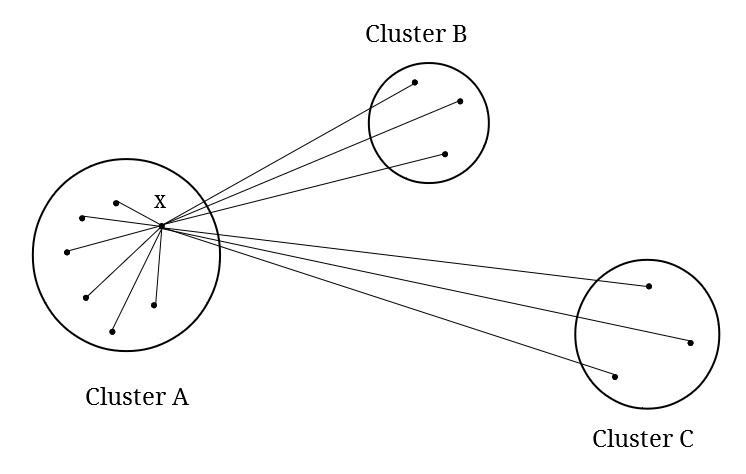
\includegraphics[width= 10cm, keepaspectratio]{pics/sil_score.jpg}
    \captionsetup{justification=centering,margin=2cm}
    \caption{Computation of silhouette score $s(x)$ with three clusters for point $x$ in cluster $A$.}
    \label{fig:sil_score}
\end{figure}


\subsubsection{Elbow Analysis}
Elbow analysis \cite{thorndike1953belongs,ketchen1996application} is another method of finding the number of clusters ($k$). The K-means algorithm works by finding the clusters which minimize the within cluster variance. The sum of squares of all the points in a cluster explains the variance within a cluster and hence it is used in elbow analysis to find the optimal number of clusters. 

Elbow analysis uses the within cluster sum of errors (WCSS). WCSS is calulated as the sum of distances of each point of a cluster and the centroid of that cluster. 

\todo{redraw the figure}
\begin{figure}[!ht]
    \centering
    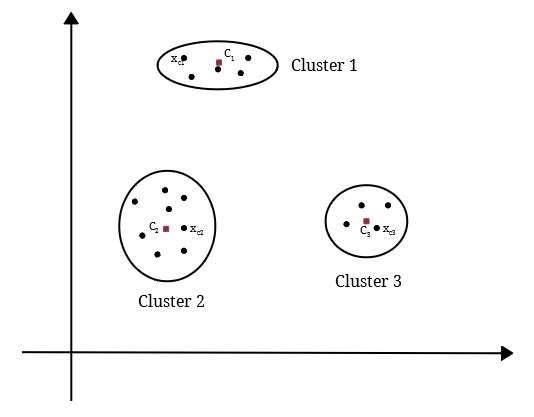
\includegraphics[width=8cm,keepaspectratio]{pics/Elbow.jpg}
     \captionsetup{justification=centering,margin=2cm}
    \caption{An illustration of clusters and centroids, with three clusters and their respective centroids $C_{1}$, $C_{2}$, $C_{3}$}
    \label{fig:elbow}
\end{figure}

For the clusters in the \ref{fig:elbow}, WCSS will be calculated as follows.
\begin{equation}
   WCSS = \sum_{i=1 }^{n}\sum_{k=1}^{n}distance(x_{i,j},C_{k})
\end{equation}

where:
\begin{align*}
      & x_{i,k}=\text{Data point $i$ in cluster $k$}\\
      & C_{k}=\text{Centroid for cluster $k$}\\
\end{align*}

This WCSS distances is plotted against the number of clusters which show an elbow shape; adding more clusters will decrease the information gain and will not model the data better.

\begin{figure}[!ht]
    \centering
    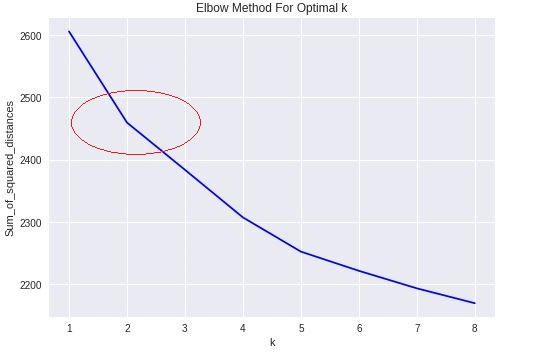
\includegraphics{pics/Elbow_example.jpg}
     \captionsetup{justification=centering,margin=2cm}
    \caption{Illustration of elbow at $k =2$ }
    \label{fig:elbow_at_2}
\end{figure}

In the \ref{fig:elbow_at_2} we can see the elbow shape at $k=2$ on the x axis. This suggest that we divide the data into two clusters.

\todo{why elbow is not trust worth and why it has to be used with silhouette scores.}

\clearpage
\section{Support Vector Machine}\label{sec:svm}
Text Categorization is an important technique for handling and organization of text corpora. The aim of categorization is the classification of text into some predefined categories. Support Vector Machines are based on \textit{Structural Risk Minimization},
which aims to find out a hypothesis $h$ for which we have the lowest \textit{true} error. The true error of $h$ is the probability that $h$ will make an error on the unseen and randomly selected data. Support Vector Machines are universal learners, also their ability to learn is independent of the dimensionality  of the input features. The dimensionality is high in case of text and also most text categorization problems are linearly separable \cite{joachims1998text}, which makes them suitable for text categorization.   

%\todo[inline]{About svm and how it works}
A Support Vector Machines is a supervised learning algorithm. It tries to find linear (in case of Linear SVM Kernel) boundaries in the given feature space. An SVM tries to maximize the distance between the two points of a decision surface \cite{manning2010introduction}.

\begin{figure}[!ht]
    \centering
    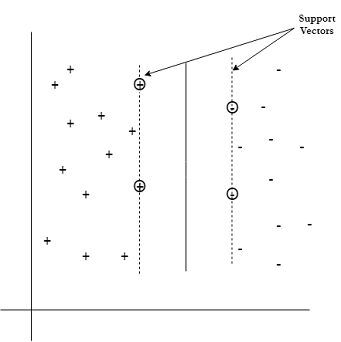
\includegraphics{pics/svm.png}
    \captionsetup{justification=centering,margin=2cm}
    \caption{Support Vector Machines}
    \label{fig:svm}
\end{figure}

 

% The following paragraph will be in the implementation chapter



\clearpage
\section{Deep Learning} \label{sec:DeepLearning}

The rise in digitization brought in the problem of creation of huge and diverse unstructured data. With the increase in computation power and the need to analyse the data to get better insight of it has given rise to deep learning. Deep learning is a sub category of artificial intelligence which is inspired by human brain and replicate the way a human learns. An Artificial Neural Network (ANN) mimics the human brain. Basic neural network will have an input layer, one output layer along with a hidden layer consisting of units that process given input into something that the output layer can use.   ANNs are incredible tools for recognizing patterns which are way too complex for programmers to extract and teach the machine to recognize.Neural Networks have been in to existence since last century, however it is during last decade they have become a major part of artificial intelligence due to the technique called backpropagation.

An artificial neuron is the building block of an ANN. Every input is multiplied with random weights so that the inputs are weighted.  These weighted inputs are then summed up with biases and passed through a transfer function and then the net input is passed through the activation function.

\begin{figure}[!ht]
    \centering
    \captionsetup{justification=centering,margin=2cm}
    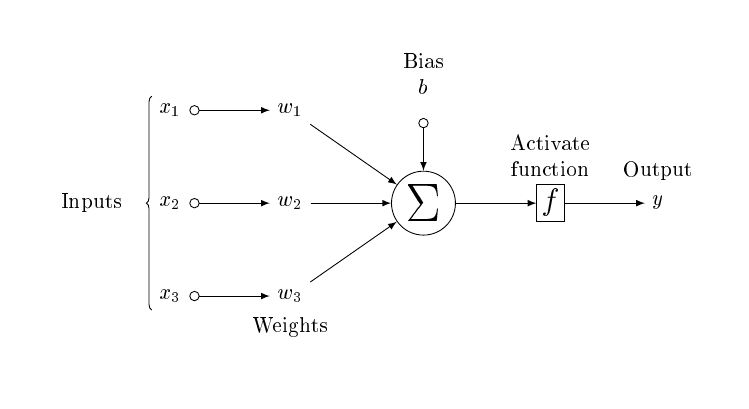
\includegraphics[width=12cm]{pics/ArtificialNeuronModel.png}
    \caption{An Artificial Neuron}
    \label{fig:neuron}
\end{figure}

The output of the neuron in the \ref{fig:neuron} would be as follows:

\begin{equation}
y=f(x_{1}w_{1}+x_{2}w_{2}+x_{3}w_{3}+b)
\label{eq:NNformula}
\end{equation}

Although the structure and computation of a single artificial neuron looks simple and easy, but its full potential and power of calculation is realized when they are interconnected and made into an artificial neural network. An artificial neural network comprises of an input layer, hidden layers and output layer as shown in \ref{fig:NN}.
\begin{figure}[!ht]
    \centering
    \captionsetup{justification=centering,margin=2cm}
    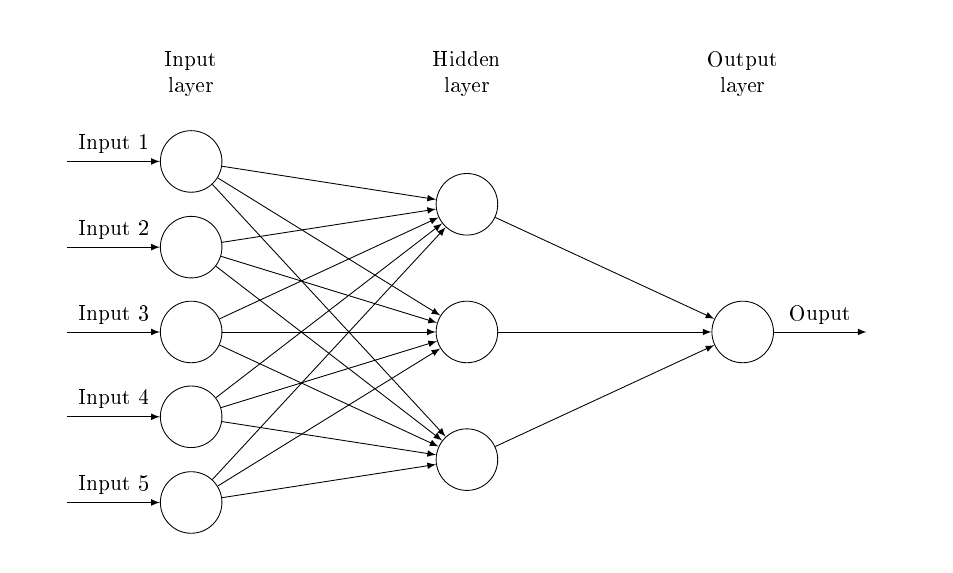
\includegraphics[width=10cm]{pics/neural_network.png}
    \caption{Artificial Neural Network}
    \label{fig:NN}
\end{figure}

A single neuron is not powerful enough to solve big and complex real world problems, but when they are put together in a specified topology or architecture they can be very handy in solving the same task a single neuron fails to do so. Advantage of artificial neural network is that these neurons can process data in distributed way, in parallel, non-linearly and locally \cite{andrej2011introduction}.
\\
\\
\\
\par
The ways in which these neurons are connected is what makes them so powerful. There are basically two main topologies in which these neurons are connected. 
\begin{figure}[!ht]%
\centering
\subfigure[Feed forward neural network]{%
\label{fig:FFRNfirst}%
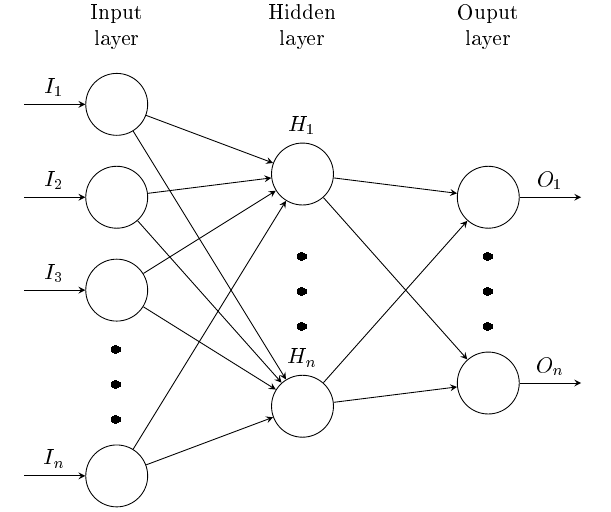
\includegraphics[height=4cm]{pics/nn2.png}}%
\qquad
\subfigure[Recurrent neural network]{%
\label{fig:FFRNsecond}%
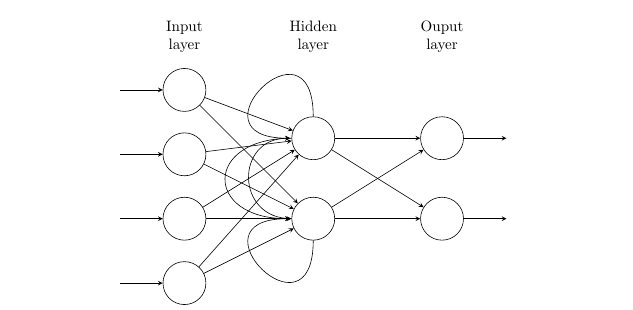
\includegraphics[height=4cm]{pics/rnn.png}}%
\caption{sample}
\label{fig:FFRN}
\end{figure}

As we can see from the \ref{fig:FFRNfirst} that in feed forward neural network the flow of information is only in one direction that is from inputs to the outputs wherein in the recurrent neural network the information flows in many possible directions as show in the  \ref{fig:FFRNsecond}

\subsection*{Activation functions}
Activation functions are important features of artificial neural networks. Activation functions is described as a function which converts the input into outputs. Consider the example of flow of current in an electric circuit as information flow in a neural network, switch in the circuit as activation function in neural network. Hence, an activation function is responsible for \textit{ON} and \textit{OFF} state of the circuit depending on the input. As the artificial neurons are inspired by the biological neuron, the activation function in biological from is either the neuron is firing or not.   

The activation function is a non linear transformation applied to the input. When the non linear transformation is not applied to the input, the output that we get would be a linear transformation, which is rather easy to solve but will not model many real world complex problems. A neural network without the activation is basically a linear regression model. The use of activation function is highly dependent on the problem at hand. Some of the most common activation functions are listed below.

\subsubsection*{Sigmoid activation function}
Sigmoid is one of the most common activation function used in neural networks. This function is widely used because its easy to calculate their derivatives, which makes weights calculation very easy in some cases. Sigmoid activation can suffer from the vanishing gradient problem.\cite{bengio1994learning}. Vanishing gradient occurs when layers of a neural network have gradients of $0$ because layers above them have saturated between -1 and 1. \cite{maas2013rectifier}


%equation of sigmoid
\begin{equation}
S(x) = \frac{1}{1+e^{-x}} \\
\label{eq:sig}
\end{equation}

\begin{figure}[!ht]
    \centering
    \captionsetup{justification=centering,margin=2cm}
    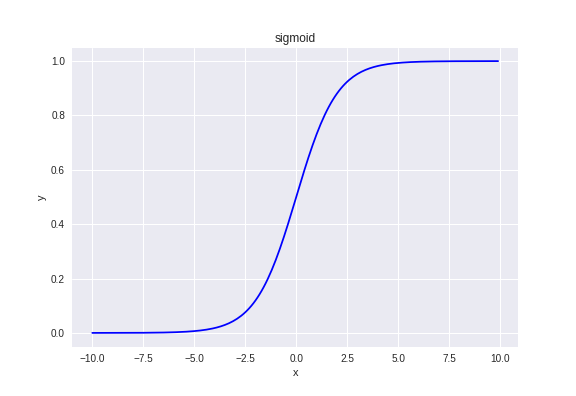
\includegraphics[width=9cm, height=9cm, keepaspectratio]{pics/sigmoid_10.png}
    \caption{Sigmoid activation function}
    \label{fig:sigmoidActivation}
\end{figure}

\subsubsection*{Rectified Linear Unit (ReLU) activation function}
The Rectified Linear Unit function is the most popular activation function from deep neural networks. The Rectified Linear Unit offers alternative nonlinearities compared to sigmoid functions, which mitigates the problem of sigmoids vanishing gradient, however during optimization procedure when these units are inactive the gardient is $0$ which leads to the problem of these units never getting activated as gradient based optimization will never adjust the weights of units which did not activate initially \cite{maas2013rectifier}\\
%equation of relu
\begin{equation}\label{eq:ReLU}
f(x) = \begin{Bmatrix}
0 & x < 0 \\ 
x & x \geq 0 
\end{Bmatrix}
\end{equation}
%graph of relu
\begin{figure}[h]
\centering
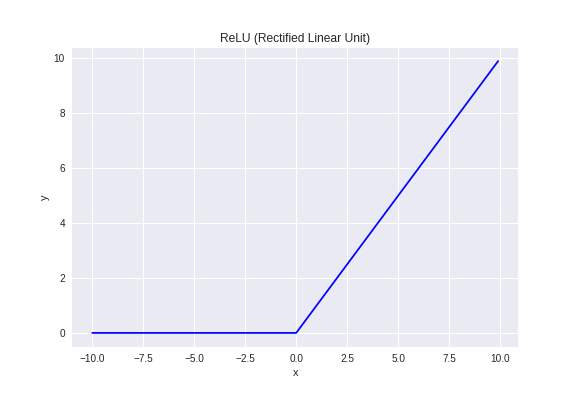
\includegraphics[width=9cm, height=9cm, keepaspectratio]{pics/ReLU_10.png}
\caption{Rectified Linear Unit Activation Function}
\label{fig:ReLU}
\end{figure} 

\subsubsection*{Hyperbolic Tangent}
This function is defined as ratio between the hyperbolic sine and hyperbolic cosine functions. Characteristics of this function is similar to sigmoid function. It outputs the values between -1 and 1 as it can be seen in the \ref{fig:tanh}

%eq 
\begin{equation}\label{eq:tanh}
f(x) = tanh(x)=\frac{2}{1+e^{-2x}} -1
\end{equation}
%fig
\begin{figure}[h]
\centering
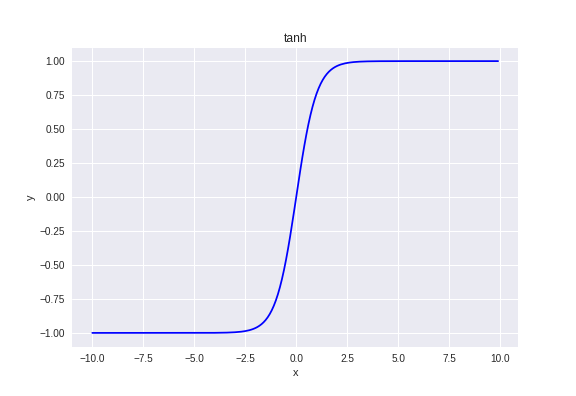
\includegraphics[width=9cm, height=9cm, keepaspectratio]{pics/tanh_10.png}
\caption{TanH Activation Function}
\label{fig:tanh}
\end{figure} 

\subsection*{Softmax activation function}
Softmax activation function is a generalization of the logistic function, in probability theory the output of the softmax function can be used to represent a categorical distribution, that is a probability distribution over \textit{X} possible outcomes. Hence, softmax activation function is used in various multi-class classification in artificial neural networks \cite{wu2016deep}.
%equation forsoftmax
\begin{equation}\label{eq:softmax}
f(x_{i}) =\frac{e^{x_{i}}}{\sum_{N=1}^{J} e^{x_{i}} }     
\end{equation}

Where:
\begin{align*}
    f(x_{i}) &= \text{Probability of $i_{th}$ class}\\
    x_{i} &= \text{$i_{th}$ dimension output}\\
    N &= \text{Total number of classes}\\
\end{align*}

\subsection{Backpropagation}\label{backprop}
\todo{check backprop example in appendix. There is mistak in calculation of backward pass}
Backpropagation is shorthand for ``backward propagation of errors". In feed forward neural network when information flows from input layer to the each hidden layer to produce the output which is refereed to as \textbf{forward propagation} or \textbf{forward pass}. This forward pass continues to produce a scalar cost that is simply the difference between target (what the network should have produced, true target) and output (what network produced). The \textbf{backpropagation} or \textbf{backward propagation} algorithm allows this cost to flow backwards in the network to compute the new weights of the network \cite{goodfellow2016deep}. It is the learning procedure which adjust the weights of the connections in a network in order to minimize the difference between input vector and the desired output vector \cite{rumelhart1988learning}.

Consider a simple neural network with one input layer with 3 inputs namely $x_{1}$, $x_{2}$ and $x_{3}$, one hidden layer consisting of 2 neurons $h_{1}$ and $h_{2}$, and one output neuron, $o_{1}$. The activation function is a sigmoid activation and the cost function is simple Euclidean distance. 

\begin{figure}[!ht]
    \centering
    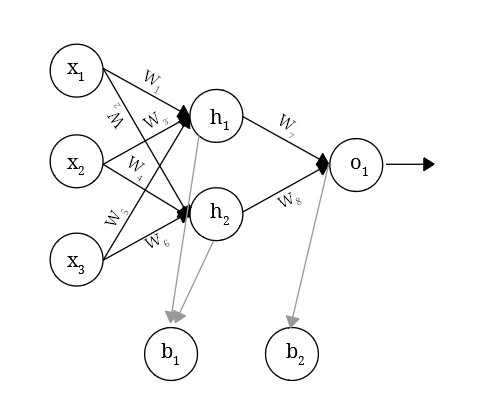
\includegraphics[width=9cm, height=6cm, keepaspectratio]{pics/backprop1.jpg}
    \caption{Single hidden layer neural network with one output}
    \label{fig:backPropExample}
\end{figure}

\subsection*{Forward pass}
In the forward pass the network will calculate the \textit{net} output of the hidden neurons, the apply the activation function to calculate the output of the hidden neurons and continue the process for the output layer neurons in the following way,
\begin{align}
    net_{h_{1}} &= (x_{1}w_{1}+x_{2}w_{3}+x_{3}w_{5}+b_{1})\\
    net_{h_{2}} &= (x_{1}w_{2}+x_{2}w_{4}+x_{3}w_{6}+b_{2})
\end{align}

Applying the activation function (sigmoid activation) to the \textit{net} output of the neurons of the hidden layers,

\begin{align}
    out_{h_{1}} &= \sigma (net_{h_{1}})\\
    out_{h_{1}} &= \frac{1}{1+e^{-net_{h_{1}}}}\\
    out_{h_{2}} &= \frac{1}{1+e^{-net_{h_{2}}}}
\end{align}
Then the \textit{net} output of the output layer is calculated by,
\begin{align}
    net_{o_{1}} &= (h_{1}w_{7}+h_{2}w_{8}+b)
\end{align}

Applying the activation function to the \textit{net} output to calculate the output of the output neuron $o_{1}$
\begin{align}
    out_{o_{1}} = \frac{1}{1+e^{-net_{o_{1}}}}
\end{align}

After the output at the output layer is obtained, the network will calculate the error or the cost function,

\begin{align}
    E_{\text(target, output)} &= \sum\frac{1}{2}(target-output)^2 \label{eq:backpropSUM} \\
    E_{total} &= E_{o_{1}} \\
    E_{total} &= \frac{1}{2}(target_{o_{1}}-out_{o_{1}})  
\end{align}

The error is calculated and this error is then used in the backward pass to calculate the new weights to be updated in order to minimize the error (Summation $\sum$ in the \ref{eq:backpropSUM} indicates that error will be calculated for each output neuron and then summed up).

\subsection*{Backward Pass}
In order to update the weights of the network, the effect to error on those weights is to be calculated, that is $\frac{\partial E}{\partial w}$, which is the rate of change of error function with respect to the weights also referred to as \textit{gradient} with respect to $w$. This is calculated by chain rule of calculus which is used to calculate the derivative of an unknown function by calculating the derivative of known functions.

The derivative of $\frac{\partial E_{total}}{\partial w_{7}}$ using chain rule is as follows,

\begin{align}
    \frac{\partial E_{total}}{\partial w_{7}} = \frac{\partial E_{total}}{\partial out_{o1}} * \frac{\partial out_{o1}}{\partial net_{o1}} * \frac{\partial net_{o1}}{\partial w_{7}} \label{eq:backPass}
\end{align}
Calculating each term individually,
\begin{align}
    \frac{\partial E_{total} }{\partial out_{o_{1}}} &= \text{change in total loss w.r.t output of $o_{1}$}
\end{align}
From , we can write,
\begin{align}
    E_{total} &= \frac{1}{2}(target_{o_{1}} - out_{o_{1}})^{2}
\end{align}

Taking the partial derivative of $E_{total}$ with respect to $out_{h_{1}}$, the part $\frac{1}{2}(target_{o_{2}} - out_{o{1}})^{2}$ becomes 0 because $out_{h_{1}}$ does not effect it and hence it is a constant.
\begin{align}
    \frac{\partial E_{total}}{\partial out_{o_{1}}} &= 2 * \frac{1}{2}(target_{o_{1}} - out_{o_{1}})^{2 - 1} \
\end{align}
Now for the second term in the equation \ref{eq:backPass}, we find out the rate of change of $out_{o_{1}}$ w.r.t $net_{o_{1}}$, hence we need to calculate the partial derivative of the sigmoid function. 
\begin{align}
    out_{o_{1}} &= \frac{1}{1-e^{net_{o_{1}}}}\\
    \frac{\partial out_{o_{1}}}{\partial net_{o_{1}}} &=  out_{o_{1}}*(1-out_{o_{1}}) \\
\end{align}
Finally, how much the $net_{o_{1}}$ changes w.r.t $w_{7}$,
\begin{align}
    net_{o_{1}} &= w_{7} * out_{h_{1}} + W_{8} * out_{h_{2}} + b_{2}   \\
    \frac{\partial net_{o_{1}}}{\partial w_{7}} &=  1 * out_{h_{1}} * w_{7}^{(1 - 1)} + 0 + 0
\end{align}

Calculating the new weight value $w_{7}$ using all the values from \ref{eq:backPass}, 

\begin{align}
    w_{7_{new}} &= w_{7} -\text{learning rate} * \frac{\partial E_{total}}{\partial w_{7}} \\ 
\end{align}

\subsection{Backpropagation Through Time}
The Backpropagation through Time (BPTT) is an extension of Backpropagation which is based on transforming a feedback network to a feedforward network by unfolding it over time \cite{ahmad2004recurrent}. Therefore, when a network processes a sequence which is $t$ times long, then $t$ copies of the network are created and the feedback connections are modified to be feedforward connections from one copy to another. This method is similar to training a large feed forward neural network with weights being modified and treated as shared weights.

\section{Text Representation}\label{backgroundTextRepresentation}

All text based computer systems requires some representation of textual data depending on the type of problem at hand. Unlike other data formats, textual data is semi structured or even unstructured. The representation of text in such system is done by transforming text into numerical form.  Detailed below are two of the most popular text representation techniques, TF-IDF and Word Embeddings.  

\subsection{Term Frequency - Document Inverse Frequency}
TF-IDF is the most common weighting method for describing textual data. Machine learning techniques such as Support Vector Machines and K Nearest Neighbours make use of this weighting scheme for text categorization. This technique works by first calculating \textit{Term Frequency} which is how often a word appears in a particular document and \textit{Inverse Document Frequency} which measure how infrequent a term is in the corpus \cite{soucy2005beyond}.

\textit{Term Frequency} is calculated as follows,

\begin{equation}\label{tf}
tf_{i,j} = \frac{n_{i,j}}{\sum_{k}n_{i,j}}
\end{equation}
where:
\begin{align*}
      & i=\text{word in the document}\\
      & j=\text{document from corpus}\\
      & k=\text{total documents in the corpus}      \\
      & n_{i,j}=\text{frequency of word $i$ in document $j$}      
\end{align*}                

Inverse Document Frequency (IDF) is a measure of importance of a word. In case of \textit{Term Frequency} all the words are considered equally important but in case of Inverse Document Frequency not all words are considered equally. While $IDF$ measures the importance of words in the corpus, some words which are referred to as \textit{stop words} such as \textit{is, of, are, the} which appear quite often in the document are of very little importance. Hence IDF will weigh less the frequently appearing words in the corpus compared to rarely appearing words. \cite{robertson2004understanding}. 

\begin{equation}\label{idf}
idf_{w} = \log\frac{N}{n_{i}}
\end{equation}
where:
\begin{align*}
      & N=\text{number of documents in corpus}\\
      & n_{i}=\text{number of documents with term $i$ in it}\\
\end{align*}     

From equation \ref{tf} and \ref{idf}, $TF-IDF$ score is computed as,

\begin{equation}\label{tf-idf}
w_{i,j} = tf_{i,j} \times \log\frac{N}{n_{i}}
\end{equation}
where:
\begin{align*}
      & tf_{i,j}=\text{number of times $i$ appears in $j$}\\
      & N=\text{number of documents in corpus}\\
      & n_{i}=\text{number of documents with term $i$ in it.}\\
\end{align*}

\subsection{Word Embeddings}
Conventionally, text representation in natural language processing involves techniques like \textit{bag-of-words} model in which a text is represented by the bag (words in the text), \textit{skip-gram} model which is generalization of \textit{n-grams} models where the words do not need to be successive for the text in consideration but can be skipped, hence named \textit{skip-gram} \cite{guthrie2006closer} and  \textit{tf-idf}. These techniques are a simple representation of various features. However, in the bag-of-words approach, grammar and word order are not considered. And in tf-idf only the importance of words is considered, \ref{sec:svm}. Hence, these techniques do not capture the semantics of the text. \cite{maas2011learning}.

Due to the above mentioned limitations, word embeddings were introduced. Word embeddings are a vector representation of the meaning of words in the corpus. This means that words are placed in a high-dimensional vector space where words with the similar meaning are placed close to each other. Neural network-based word vector models are usually trained using stochastic gradient descent where the gradient is obtained by backpropagation \cite{le2014distributed}.

To better understand how word vectors are employed, we consider an example of reviews of cars from 0 to 5 in various categories, where 0 is worst and 5 is best category. Lets say a car ``Volkswagen beetle" scores 3 on comfort (one of the evaluation criteria). Representing it on a scale and converting it from range 0 to 5 to 1 to -1.

\begin{figure}[!ht]
    \centering
    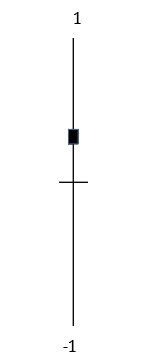
\includegraphics[width=2cm]{pics/wordVec.jpg}
    \captionsetup{justification=centering,margin=2cm}
    \caption{Comfort of ``Volkswagen beetle" on scale of 0-5, rescaled to range -1 to 1}
    \label{fig:volkswagan_example}
\end{figure}

Now this does not consider all the aspect of this approach. So, consider another evaluation criterion leg room (amount of space for your legs). Beetle has scored 4 in the leg room category. hence we represent it on a scale of -1 to 1 and add another dimension which represents the leg room category. 

\begin{figure}
    \centering
    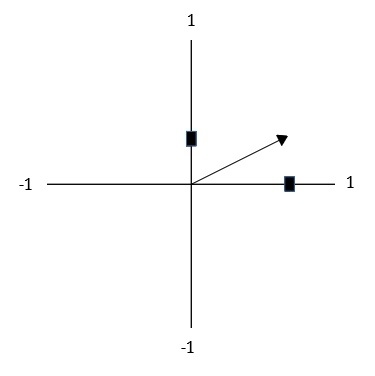
\includegraphics[width=5cm]{pics/wordVec_2.jpg}
    \captionsetup{justification=centering,margin=2cm}
    \caption{Comfort represented on x-axis and leg room on y-axis}
    \label{fig:volkswagan_example_2}
\end{figure}

Adding a few other cars we have a vector representation of those cars in a multi dimensional space (represented here in two dimensional space) \ref{fig:wordVecManyCars}


\begin{figure}[!ht]
    \centering
    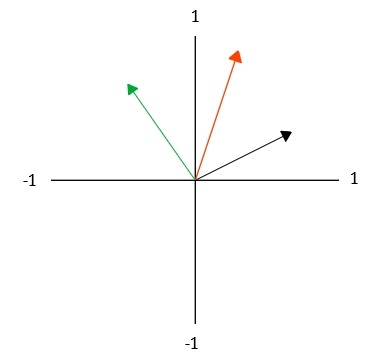
\includegraphics[width=5cm]{pics/wordVec_2_manycars.jpg}
    \captionsetup{justification=centering,margin=2cm}
    \caption{Vector representation of car features in a two dimensional space, black represents Volkswagen, red represents Mercedes and green represents Audi}
    \label{fig:wordVecManyCars}
\end{figure}


Using vectors, we can easily find the similarity between two cars using \textit{cosine similarity}.

\begin{table}[!ht]
\centering
\begin{tabular}{cc}
\hline
\textbf{Cars} & \textbf{Vectors} \\ \hline
Volkswagen    & 0.2, 0.4         \\ \hline
Mercedes      & 0.1, 0.6         \\ \hline
Audi          & -0.3, 0.5        \\ \hline
\end{tabular}
\caption{Vectors of cars}
\captionsetup{justification=centering,margin=2cm}
\label{my-label}
\end{table}

\begin{equation}
        \text{cosine-similarity (Volkswagen, Mercedes)} = 0.955 
\end{equation}
\begin{equation}
    \text{cosine-similarity (Volkswagen, Audi)} = 0.536
\end{equation}
\begin{equation}
    \text{cosine-similarity (Mercedes, Audi)} = 0.761
\end{equation}

Adding more dimensions captures more information and hence increases the quality of the results. These vectors represent the cars with numbers which is necessary for machines to understand and also we can calculate similarities between these vectors. 

One popular algorithm is \textbf{Word2Vec} \cite{mikolov2013efficient}, in this implementation word embeddings are trained using two models, \textit{continuous bag-of-words} model and \textit{continuous skip-gram model}. In continuous bag-of-words, the projection of words into the vector space is not influenced by the order of words and words from the future are also used in this model. In the Continuous Skip-gram model, instead of predicting next word based on the context, it tries to maximize the classification of next word based on other word in the fixed window size sentence.

Consider the following sentence to understand how the aforementioned methods works,

\begin{quote}
    \textit{I am the master of my fate, I am the captain of my soul} - Invictus, William Ernest Henley.
\end{quote}

\subsubsection*{Continuous Bag-of-words Model}
This model works by looking at words not only from a few words in the past but also a few words from the future to predict the target word. 

\begin{figure}[!ht]
    \centering
    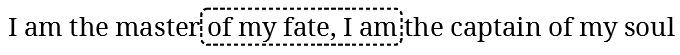
\includegraphics[width=12cm]{pics/bag-of-wordWord2Vec.jpg}
    \caption{Continuous bag-of-words model data set creation}
    \label{fig:word2VecBagOfWords}
\end{figure}

The target word is \textit{``fate"} and we want to predict it so we take a sliding window over the sentence as shown in \ref{fig:word2VecBagOfWords}. 

\begin{table}[!ht]
\centering
\begin{tabular}{ccccc}
\hline
\multicolumn{1}{l}{\textbf{Input 1}} & \multicolumn{1}{l}{\textbf{Input 2}} & \textbf{Input 3} & \multicolumn{1}{l}{\textbf{Input 4}} & \textbf{Output} \\ \hline
i & am & master & of & the \\ \hline
am & the & of & my & master \\ \hline
the & master & my & fate & of \\ \hline
master & of & fate & i & my \\ \hline
of & my & i & am & fate \\ \hline
\end{tabular}
\caption{Dataset for training continuous bag-of-words model}
\label{datasetBagOfWords}
\end{table}

This process will continue for the whole sentence in this case and whole corpus in case we have a big dataset. This dataset will then be feed into neural network for it to learn. 

\subsubsection*{Continuous Skip-gram Model}
This model tries to predict the neighbouring words based on the current word. So the training process for the above mentioned sentence is as follows.

We can take a sliding window over the sentence and construct a dataset for training the skip-gram model, 
\begin{figure}[!ht]
    \centering
    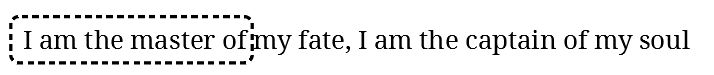
\includegraphics[width=12cm]{pics/skipgramWord2vec.jpg}
    \caption{Continuous skip-gram model dataset creation}
    \label{fig:skipgramWord2vec}
\end{figure}

We take the word \textit{``the"} and then start building the dataset as the word \textit{``the"} as input and the two left neighboring words \textit{``i"} and \textit{``am""} and the two right neighboring words \textit{``master"} and \textit{``of"} as shown in the \ref{fig:skipgramWord2vec}

\begin{table}[!ht]
\centering
\begin{tabular}{cc}
\hline
\textbf{Input} & \textbf{Output} \\ \hline
the            & i               \\ \hline
the            & am              \\ \hline
the            & master          \\ \hline
the            & of              \\ \hline
\end{tabular}
\caption{Dataset for training continuous skip-gram model}
\label{word2vec-skipgram-dataset}
\end{table}

This process will continue for the whole sentence until each and every word of the sentence is in the training dataset against its neighboring words. This dataset is then feed to the untrained neural network to predict the output.  

After the network converges, words with similar meaning are placed together in the embedding space. For example words like "powerful" and "strong" are placed close to each other in the vector space. \todo{Need to work on this, doesn't look good}


\todo{This following paragraph goes into implementation}

The model used in creation of the word vectors is a neural network, and neural networks are data hungry as it requires a lot of data to train them properly. As a result, another domain specific dataset is used in this experiment because dataset used for classification is small. Hence, the whole EUR-Lex dataset was used as it contains 19,348 documents mostly consisting regulations, decisions and directives of European Union \cite{jf:SemanticLaw}.

\subsection{Cross Lingual Word Embedding}\label{backgroundCrosslingual}

Word vectors for different languages are in different vector spaces, hence it can not be combined together, but the classification task involves classifying text from two languages, \textbf{English} and \textbf{German}. Hence, for classifying both languages within a single model is necessary. This not only mitigates the error caused by a language detector in multilingual systems, where a language detector first detects the language and then the respective classifier is invoked. In that affair, error propagates downwards and amplifies. And using multiple languages also increase the amount of data for training if multilingual parallel corpora is available where corpus of single language is low. 

To achieve this Duong et. al \cite{duong-EtAl:2016:EMNLP}, proposed using bilingual dictionaries and monolingual data. The model uses an extension of contextual bag-of-word(CBOW) model \cite{mikolov2013efficient}. This method has benefits as often there no parallel data when working on a domain specific problems, also it is comparatively easy to obtain or create bilingual domain specific dictionaries.

Facebook's MUSE Python library \cite{conneau2017word} aligns word vectors from multiple languages to a single vector space, the author claims that these embeddings state-of-art multilingual word embeddings, they have used Facebook's Fasttext \cite{bojanowski2017enriching} monolingual word embeddings and aligned them in common vector space. They use two sets word embeddings that are trained on monolingual data, and learns the mapping between these two embedding in a common vector space. It exploits the similarities of monolingual embedding space \cite{mikolov2013exploiting} to learn mapping between the two embeddings.

\subsection{Long Short Term Memory}
Neural networks have shown remarkable capabilities in processing and modeling natural language. Recurrent Neural Networks (RNN) and Convolutional Neural Networks (CNN) are common architectures for handling natural language. Long Short Term Memory (LSTM)\cite{hochreiter1997long} is a variant of RNNs, unlike other feed forward neural networks these networks have recurrent connections in them which allow information to persist.

\begin{figure}[!ht]
    \centering
    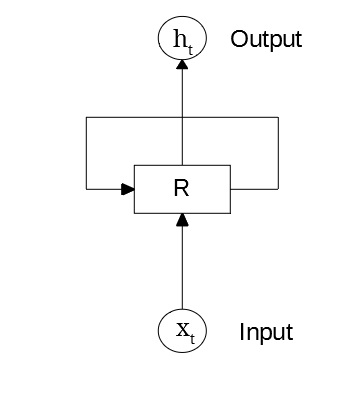
\includegraphics[width=4cm,height=6cm,keepaspectratio]{pics/rnn_cell.jpg}
    \captionsetup{justification=centering,margin=2cm}
    \caption{Single RNN Cell}
    \label{fig:rnn_single_cell}
\end{figure}

The \ref{fig:rnn_single_cell} shows a single RNN cell having a recurrent connection. This recurrent connection allows it to retain the previous state and make use of the context of the previous state \cite{graves2009novel}. Due to this property RNNs are very effective in processing text. 

RNNs are effective but suffer from the problem that the capacity of them to retain the previous states is fairly limited. The problem is that the input influences either diminishes the output or increases it exponentially. This is referred to as the problem of \textit{vanishing gradients}\cite{hochreiter2001gradient}. This problem makes it hard for RNNs to make use of more than a few previous states. LSTMs are a special kind of RNNs which address the problem of vanishing gradients. They contains recurrently connected sub-networks called \textit{memory blocks} and each of these blocks contains three gates; input gate, forget gate and output gate. These gates allows an LSTM to store information for a longer period of time. If the input gate is shut, that is if it has no activation (or close to 0), the activation of a block will not be overwritten for the next incoming inputs. Also, the block activation is only available to the network when the output gate is open. The forget gate switches on and off the recurrent connections.

\begin{figure}[!htbp]
    \centering
    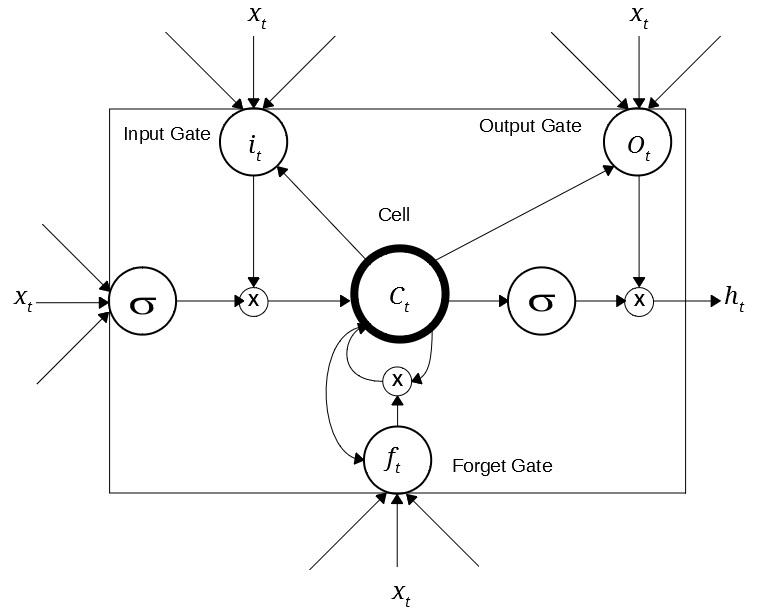
\includegraphics[width=10cm]{pics/lstm.jpg}
    \captionsetup{justification=centering,margin=2cm}
    \caption{LSTM block with a single cell. The cell has recurrent connections with a forget gate. The three gates collect inputs from rest of the network. }
    \label{fig:LSTM_BLOCK}
\end{figure}


Let $X$ $=$ ${x_{1}, x_{2},....,x_{n}}$ be the input sequence and $Y$ $=$ ${y_{1}, y_{2},....,y_{n}}$ be the output sequence. An LSTM network learns the mapping of input sequence to the output sequence using the following equations one by one from time $t$ $=$ 1 to $n$. Hence, the equation for the respective gates and the cell states are as follows:

\begin{equation} \label{eq:lstm_input_gate}
    i_{t} =\sigma(w_{i}[h_{t-1},x_{t}]+b_{i})
\end{equation}
\begin{equation}\label{eq:lstm_forget_gate}
    f_{t} =\sigma(w_{f}[h_{t-1},x_{t}]+b_{f})
\end{equation}
\begin{equation}\label{eq:lstm_output_gate}
    o_{t} = \sigma(w_{o}[h_{t-1},x_{t}]+b_{o})
\end{equation}

where:
\begin{align*}
      & i_{t}=\text{input gate}\\
      & f_{t}=\text{forget gate}\\
      & o_{t}=\text{output gate}\\
      & \sigma=\text{sigmoid function}\\
      & W_{i}=\text{Weight matrix of input gate}\\
      & W_{f}=\text{Weight matrix of forget gate}\\
      & W_{o}=\text{Weight matrix of output gate}\\
      & h_{t-1}=\text{output from previous block at time $t-1$}      \\
      & b_{i}=\text{bias for input gate}    \\
      & b_{i}=\text{bias for forget gate}    \\
      & b_{i}=\text{bias for output gate}\\
\end{align*}

The \ref{eq:lstm_input_gate} is for the input gate which allows whatever new information is to be stored in the cell state. \ref{eq:lstm_forget_gate} is for the forget gate which is responsible for discarding information that is not useful anymore from the cell state. \ref{eq:lstm_output_gate} is for the output gate which is responsible for the activation of the whole LSTM block at time $t$ 


\begin{equation}\label{eq:lstm_newCellState}
    \Tilde{c}_{t} =\tanh(w_{c}[h_{t-1},x_{t}]+b_{c})
\end{equation}
\begin{equation} \label{eq:lstm_CurrentCellState}
    c_{t} = f_{t} \odot c_{t-1} + i_{t} \odot \Tilde{c}
\end{equation}
\begin{equation}\label{eq:lstm_output}
    h_{t} = o_{t} \odot \tanh(c_{t})
\end{equation}
where:
\begin{align*}
      & \Tilde{c_{t}}=\text{new contender for cell state at $t$}\\
      & c_{t}=\text{current cell state at $t$}\\
      & \odot=\text{element wise product}
\end{align*}


% Yes I too thought so but I saw it is being done already
At any given time step, the current cell state knows what is to be forgotten, that is $f_{t}\odot c_{t-1}$ from \ref{eq:lstm_CurrentCellState} and which new cell state to be established from the current time step, that is $i_{t}\odot \Tilde{c}$ form \ref{eq:lstm_CurrentCellState}. This is then passed through a $\tanh$ function to filter out which of the two should be forgotten and which should be the output at the current time step. The output $h_{t}$ can then be passed through a softmax function to get the prediction probabilities for the current block.




\section{Bidirectional LSTM}
Bidirectional LSTMs are  able to access the context of a given sequence in both direction(forward and backward) \cite{schuster1997bidirectional}. In \ref{fig:BiLSTM} we can see that Bidirectional LSTM contains two layers out of which one processes the sequence in forward direction and one processes the sequence in backward direction. The output layer is connected to both layers which enables it to process both forward or future context and backward or past context. Bidirectional LSTMs have show to preformed better then standard LSTMs and RNNs in sequence learning data \cite{baldi2000bidirectional} \cite{fukada1999phoneme}.

\begin{figure}[!ht]
    \centering
    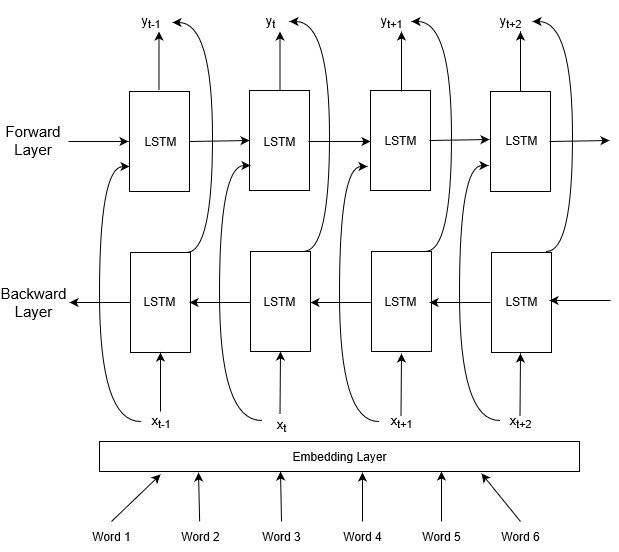
\includegraphics[width=12cm,height=8cm,keepaspectratio]{pics/BiLSTM.jpg}
    \captionsetup{justification=centering,margin=2cm}
    \caption{Bidirectional LSTM }
    \label{fig:BiLSTM}
\end{figure}

From \ref{fig:BiLSTM}, it can be seen that there is no connection between the forward passing layer and backward passing layer, hence outputs from forward pass is not connected to the input of backward class and vice versa, so training a Bidirectional LSTM is same as unidirectional LSTM for the most part.

\section{Data Distribution}
There are many inconsistencies when it comes to the number of documents in the classes. In the class \textit{justice freedom and security} there are \textit{320} documents for English corpus and \textit{314} documents for German corpus. These irregularities are of less importance when it comes to learning them separately, but becomes important when both languages are to be learned together. Information can leak from training to testing set leading to unrealistic results if these inconsistencies are not dealt with earlier. 

\begin{figure}[!ht]
\begin{center}
\makebox[2pt]{
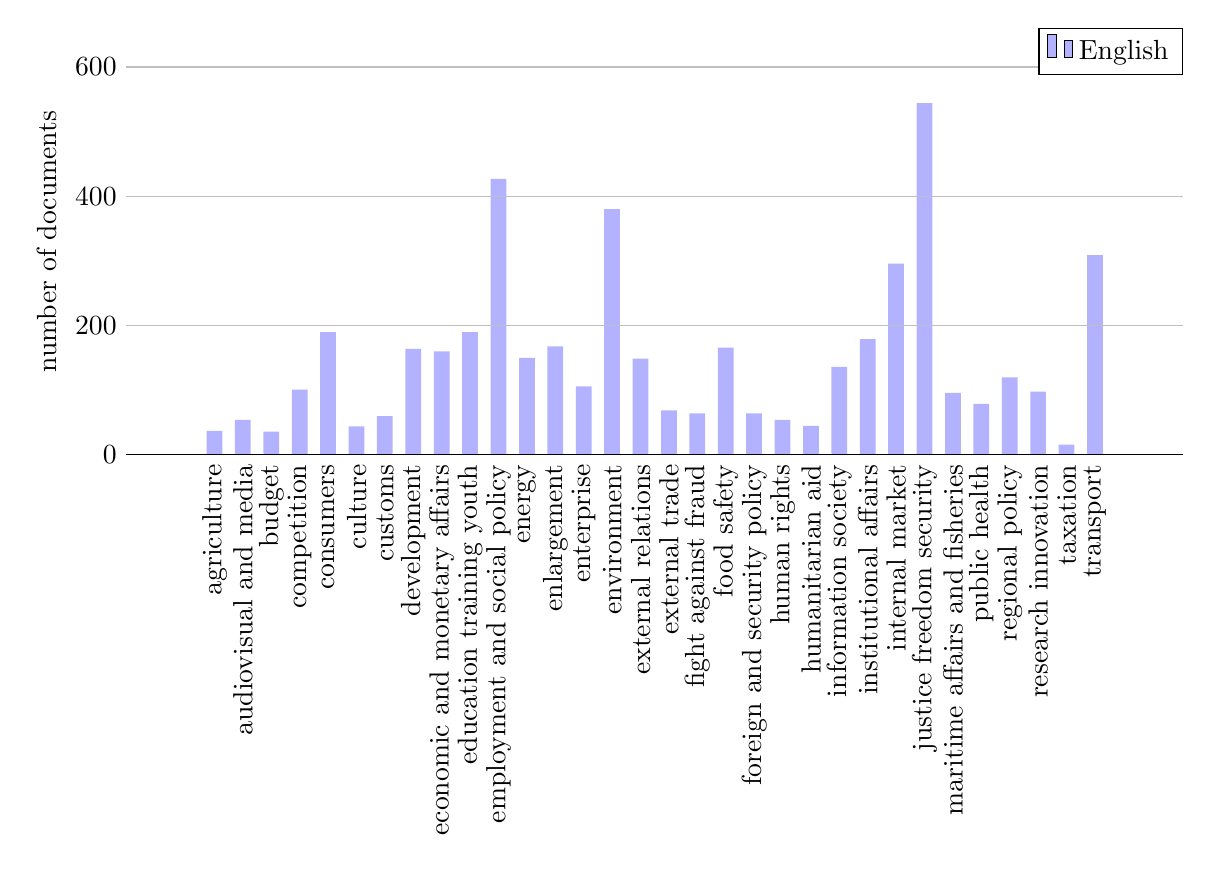
\begin{tikzpicture}
  \centering
  \begin{axis}[
        ybar, axis on top,
        title={},
        height=7cm, width=15cm,
        bar width=0.2cm,
        ymajorgrids, tick align=inside,
        enlarge y limits={value=.1,upper},
        ymin=0, ymax=600,
        axis x line*=bottom,
        axis y line*=left,
        y axis line style={opacity=0},
        tickwidth=0pt,
        ytick style={draw=none},
        enlarge x limits=true,
        legend style={
            at={(1,1)},
            anchor=north east,
            legend columns=-1,
            /tikz/every even column/.append style={column sep=0.1cm}
        },
        ylabel={number of documents},
        symbolic x coords={
        agriculture,
        audiovisual  and  media,
        budget,
        competition,
        consumers,
        culture,
        customs,
        development,
        economic  and  monetary  affairs,
        education  training  youth,
        employment  and  social  policy,
        energy,
        enlargement,
        enterprise,
        environment,
        external  relations,
        external  trade,
        fight  against  fraud,
        food  safety,
        foreign  and  security  policy,
        human  rights,
        humanitarian  aid,
        information  society,
        institutional  affairs,
        internal  market,
        justice  freedom  security,
        maritime  affairs  and  fisheries,
        public  health,
        regional  policy,
        research  innovation,
        taxation,
        transport
        },
       xtick=data,
       x tick label style={rotate=90,anchor=east},
       %nodes near coords={\pgfmathprintnumber[precision=0]{\pgfplotspointmeta}}
    ]
    \addplot [draw=none, fill=blue!30] coordinates {
        (agriculture, 37)
	    (audiovisual and media,54) 
		(budget,36) 
		(competition,101) 
		(consumers,190) 
		(culture,44) 
		(customs,60) 
		(development,164) 
		(economic and monetary affairs,160) 
		(education training youth,190) 
		(employment and social policy,427)
		(energy,150)
		(enlargement,168)
		(enterprise,106)
		(environment,380)
		(external relations,149)
		(external trade,69)
		(fight against fraud,64)
		(food safety,166)
		(foreign and security policy,64)
		(human rights,54)
		(humanitarian aid,45)
		(information society,136)
		(institutional affairs,179)
		(internal market,296)
		(justice freedom security,544)
		(maritime affairs and fisheries,96)
		(public health, 79)
		(regional policy,120)
		(research innovation,98)
		(taxation,16)
		(transport,309)  };
   
\legend{English}
\end{axis}
\end{tikzpicture}
}
\end{center}
\caption{Distribution of documents across English Language for EUR-Lex Summaries}
\label{graph:distribution of data english docs}
\end{figure}


\section{Class Imbalance}\label{backgroundImbalance}
Class imbalance occurs when the number of samples in one class is more than the other. \ref{graph:distribution of data english docs} shows that there is class imbalance in the dataset. This has to be taken into consideration before the selection of learning algorithm. Ideally, the number of samples in each class should be roughly same in order for a leaning algorithm to distinguish between them. If they are not nearly same the learning algorithm will favour the majority class and not learn the minority class. It creates \textit{accuracy paradox} which arise in such situation. For example, in a data set of 100 samples, 90 samples belonging to class $A$ and 10 belonging to class $B$, the training algorithm will naively predict everything in class $A$ which will result in accuracy of $90\%$, which is misleading. These situations are common in most machine learning problems and there are a few ways to tackle them. 


\begin{itemize}
  \item Collect more data, which is impossible in most cases.
  \item Resample the data set, which could be challenge if the data set is limited in the first place.
  \item Changing the performance metric to get more insights of the model.
  \item Penalize the algorithm through class weights.
\end{itemize}

\section{Sentence based approach for training LSTMs} \label{backgroundSlidingWindow}

Documents containing legal text are often very long. To process such documents it can divided into smaller sub-texts which are easy to process. In \cite{volkovich2016text}, authors have divided text into sub-text to consider the dependencies between written text. These long text can be processed and used theoretically by LSTMs \cite{hochreiter1997long} , it is often limited by hardware. Various techniques have been studied and applied on textual data on various levels. Text data has been annotated on different levels, on document level \cite{macdonald2006trec}, on paragraph level \cite{ferguson2009exploring}, on sentence level \cite{santos2009integrating, seki2008overview} and on the phrase level \cite{wilson2005recognizing}

To overcome this, \textit{Sliding Window} based approach is used here. A sliding window algorithm divides a long array or stream into smaller chunks.  

Consider an example to understand how slides are created on a famous quote by Mahatma Gandhi - \textit{``A man is but the product of his thoughts; what he thinks, he becomes.''}

\begin{figure}[!ht]
    \centering
    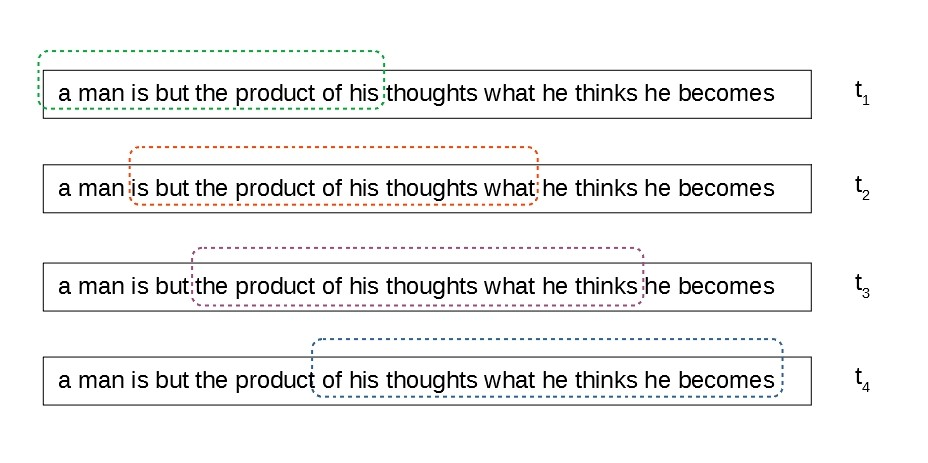
\includegraphics[width=12cm]{pics/SlidingWindow.jpg}
    \captionsetup{justification=centering,margin=2cm}
    \caption{Sliding window at time step $t_{1}$, $t_{2}$, $t_{3}$ and $t_{4}$ with the window size of 10 words per sentence and slide of 2 word per sentence per time step}
    \label{fig:sldingwindow}
\end{figure}

\ref{fig:sldingwindow} shows sliding window, with a window size of 10 words per sentence and slide of 2 words per sentence to create four sentences at time step $t_{1}$, $t_{2}$, $t_{3}$ and $t_{4}$. The following is the list of sentences that the algorithm will create with the above mentioned configuration.

\begin{itemize}
    \item Sentence 1 at time step $t_{1}$: a man is but the product of his
    \item Sentence 2 at time step $t_{2}$: is but the product of his thoughts what
    \item Sentence 3 at time step $t_{3}$: the product of his thoughts what he thinks
    \item Sentence 1 at time step $t_{4}$: of his thoughts what he thinks he becomes
\end{itemize}

In the case when there are less words left than the specified length of the window, then the process will halt with the remaining words in the last sentence.

Here, for training LSTM models, the sliding window based approach is used to create sentences out of the document. The length of slide or the resulting sentence is 30 with slide of 10 words. As each document belongs to one class, the sentences are given the same label as the document is, so if  \textbf{Doc A} $\rightarrow$  \textbf{Class 1} then all the sentences of that corresponding document will be labeled as \textbf{Class 1}. This also helps in mitigation of the problem of less data for training as a single document of 1000 if divided into sentence with sliding window then 98 sentence would be created, which means 98 instances of the class rather than 1 single document. 


\section{Evaluation Matrices}\label{backgroundEvaluationMatrices}

The evaluation of a classification model is very essential. Evaluation of a model gives us insights on how the model will if put to use in production. The following is the list of evaluation measures used in this thesis to evaluate the performance of the models. 

In order to evaluate the performance of any multi-class classification model, we need to first understand the \textit{confusion matrix}.

A confusion matrix describes the performance of a classification model on a set of data where true answers for that data is known.


\begin{table}[!ht]
\centering
\begin{tabular}{ll|l|l|}
\cline{3-4}
 &  & \multicolumn{2}{c|}{Actual Values} \\ \cline{3-4} 
 &  & \multicolumn{1}{c|}{\textbf{P}} & \multicolumn{1}{c|}{\textbf{N}} \\ \hline
\multicolumn{1}{|l|}{} & \multicolumn{1}{c|}{\textbf{P}} & True Positive & False Positive \\ \cline{2-4} 
\multicolumn{1}{|l|}{\multirow{-2}{*}{Predicted Values}} & \textbf{N} & False Negative & True Negative \\ \hline
\end{tabular}
\caption{Confusion Matrix}
\label{table:confMatrix}
\end{table}

\begin{itemize}
    \item \textbf{Positive (P)}:Positive condition (e.g. is mango)
    \item \textbf{Negative (N)}:Negative condition (e.g. is not a mango)
    \item \textbf{True Positive (TP)}: Number of samples that were Positive  (\textbf{P}) and identified and as Positive (\textbf{P}) by the algorithm.
    \item \textbf{False Positive (FP)}: Number of samples that were Negative (\textbf{N}) but identified as Positive  (\textbf{P}) by the algorithm.
    \item \textbf{True Negative (TN)}: Number of samples that were Negative (\textbf{N}) and predicted as Negative (\textbf{N}) by the algorithm.
    \item \textbf{False Negative (FN)}: Number of samples that were Positive (\textbf{P}) but identified as Negative (\textbf{N})
\end{itemize}


\subsection*{Accuracy}
Accuracy of is the ratio of number of correctly identified instances of all classes over the total number of instances in the dataset. 
\begin{align}
    Accuracy &= \frac{\text{Number of correct predictions}}{\text{Total number of predictions}}\\
    Accuracy &= \frac{TP+TN}{TP+TN+FP+FN}
\end{align}

Accuracy in case of unbalanced dataset is not a good measure to evaluate the performance of a model (See \ref{backgroundImbalance}). Hence, other evaluation matrices have to be used in order to get the per class performance of a classifier.

\subsection*{Precision}
Informally, precision indicates how many of Positive conditions were identified correctly. Formally, it is the ratio of True Positive (TP) and sum of True Positive (TP) and False Positive (FP).

\begin{align}
    Precision &= \frac{\text{Correctly identified positive conditions}}{\text{Total number of positive conditions}}\\
    Precision &= \frac{TP}{TP+FP}
\end{align}

\subsection*{Recall}
Recall also known as True positive rate is the amount of positive values that are correctly identified, that is the ratio of True Positive (TP) and sum of True Positive (TP) and False Negative (FN)

\begin{align}
    Recall &= \frac{\text{Correctly identified positive conditions}}{\text{Total number of positive prediction by algorithm}}\\
    Recall &= \frac{TP}{TP+FN}
\end{align}

\subsection*{F-measure (F1-Score)}
F-measure is the harmonic mean of the precision and recall. Harmonic mean is one of the several averaging strategies applicable in situation where average of rates is needed. It is expressed in terms of precision and recall as following,

\begin{align}
    \text{F-measure (F1-Score)} &= \left (\frac{precision^{-1} * recall^{-1}}{2}  \right ) \\
    \text{F-measure (F1-Score)} &= 2 * \frac{precision * recall}{precision + recall}
\end{align}

\subsection*{Macro and Micro Averages}

Precision, Recall and F-measure will give us the performance of the classifier on individual classes and to represent the performance of the classifier on the whole dataset we need to average this values across all the classes. The problem with averaging the values of precision, recall and f-measure across all the classes in case of imbalance of the dataset is misleading as it will weigh each class equally even though the number of samples in some classes were higher and the effect of these classes on precision, recall and f-score will be more. 

Consider the following example:
\begin{itemize}
    \item Class A: 5 TP and 5 FP
    \item Class B: 1 TP and 1 FP
    \item Class C: 20 TP and 90 FP
    \item Class D: 10 TP and 10 FP
\end{itemize}

Calculation precision on these classes we get, $P_{A}, P_{B}, P_{D}= 0.5$ and $P_{C} = 0.2$. 
In macro-average, first the individual precision is calculated and then the average is taken \cite{manning2009introduction}, so macro-average is:
\begin{align}
    \text{macro-average precision} = \frac{0.5+0.5+0.5+0.18}{4} = 0.42
\end{align}
The problem is quite clear as class C which is 84\% of the total dataset is represented in the macro-average precision by $\frac{1}{4}$ ratio \cite{manning2009introduction}.

To mitigate this, in micro-average, we sum up all the prediction of all the classes and then compute the average.
So, micro-average precision for the above example would be:
\begin{align}
    \text{micro-average precision} = \frac{5+1+20+10}{10+2+110+20} = 0.2535
\end{align}
%- Allgemeine Wissensgrundlagen des Fachgebiets
%- Spezielle Grundlagen, die für das Verständnis erforderlich sindhttps://www.overleaf.com/project/5bf3df67d5a222068c001d80
%- Rahmenbedingungen für die Arbeit
%- Ausführungen zum Stand des Wissens / der Technik
%Als Leitprinzip gilt: Nur Informationen erwähnen, die
%- später benötigt werden,
%- notwendig sind, um die Arbeit oder ihre Motivation zu verstehen
%Das heißt insbesondere,
%- keine Inhalte aus Lehrbüchern, außer
%- diese werden benötigt, um Problemstellung oder Lösungsweg zu definieren.

%\hint{The first paragraph should be introduction of things that have been already been done and how the things or techniques that I am using in this thesis may or might have helped  in similar situations. }

%\todots